\documentclass[12pt]{article}

\usepackage{amsmath, mathtools}
\usepackage{amsfonts}
\usepackage{amssymb}
\usepackage{graphicx}
\usepackage{colortbl}
\usepackage{xr}
\usepackage{hyperref}
\usepackage{longtable}
\usepackage{xfrac}
\usepackage{tabularx}
\usepackage{float}
\usepackage{siunitx}
\usepackage{booktabs}
\usepackage{caption}
\usepackage{pdflscape}
\usepackage{afterpage}

\usepackage[round]{natbib}

%\usepackage{refcheck}

\hypersetup{
    bookmarks=true,         % show bookmarks bar?
      colorlinks=true,       % false: boxed links; true: colored links
    linkcolor=red,          % color of internal links (change box color with linkbordercolor)
    citecolor=green,        % color of links to bibliography
    filecolor=magenta,      % color of file links
    urlcolor=cyan           % color of external links
}

%% Comments

\usepackage{color}

\newif\ifcomments\commentstrue %displays comments
%\newif\ifcomments\commentsfalse %so that comments do not display

\ifcomments
\newcommand{\authornote}[3]{\textcolor{#1}{[#3 ---#2]}}
\newcommand{\todo}[1]{\textcolor{red}{[TODO: #1]}}
\else
\newcommand{\authornote}[3]{}
\newcommand{\todo}[1]{}
\fi

\newcommand{\wss}[1]{\authornote{blue}{SS}{#1}} 
\newcommand{\plt}[1]{\authornote{magenta}{TPLT}{#1}} %For explanation of the template
\newcommand{\an}[1]{\authornote{cyan}{Author}{#1}}

%% Common Parts

\newcommand{\progname}{ProgName} % PUT YOUR PROGRAM NAME HERE
\newcommand{\authname}{Team \#, Team Name
\\ Student 1 name and macid
\\ Student 2 name and macid
\\ Student 3 name and macid
\\ Student 4 name and macid} % AUTHOR NAMES                  

\usepackage{hyperref}
    \hypersetup{colorlinks=true, linkcolor=blue, citecolor=blue, filecolor=blue,
                urlcolor=blue, unicode=false}
    \urlstyle{same}
                                


% For easy change of table widths
\newcommand{\colZwidth}{1.0\textwidth}
\newcommand{\colAwidth}{0.13\textwidth}
\newcommand{\colBwidth}{0.82\textwidth}
\newcommand{\colCwidth}{0.1\textwidth}
\newcommand{\colDwidth}{0.05\textwidth}
\newcommand{\colEwidth}{0.8\textwidth}
\newcommand{\colFwidth}{0.17\textwidth}
\newcommand{\colGwidth}{0.5\textwidth}
\newcommand{\colHwidth}{0.28\textwidth}

% Used so that cross-references have a meaningful prefix
\newcounter{defnum} %Definition Number
\newcommand{\dthedefnum}{GD\thedefnum}
\newcommand{\dref}[1]{GD\ref{#1}}
\newcounter{datadefnum} %Datadefinition Number
\newcommand{\ddthedatadefnum}{DD\thedatadefnum}
\newcommand{\ddref}[1]{DD\ref{#1}}
\newcounter{theorynum} %Theory Number
\newcommand{\tthetheorynum}{T\thetheorynum}
\newcommand{\tref}[1]{T\ref{#1}}
\newcounter{tablenum} %Table Number
\newcommand{\tbthetablenum}{T\thetablenum}
\newcommand{\tbref}[1]{TB\ref{#1}}
\newcounter{assumpnum} %Assumption Number
\newcommand{\atheassumpnum}{P\theassumpnum}
\newcommand{\aref}[1]{A\ref{#1}}
\newcounter{goalnum} %Goal Number
\newcommand{\gthegoalnum}{P\thegoalnum}
\newcommand{\gsref}[1]{GS\ref{#1}}
\newcounter{instnum} %Instance Number
\newcommand{\itheinstnum}{IM\theinstnum}
\newcommand{\iref}[1]{IM\ref{#1}}
\newcounter{reqnum} %Requirement Number
\newcommand{\rthereqnum}{P\thereqnum}
\newcommand{\rref}[1]{R\ref{#1}}
\newcounter{nfrnum} %NFR Number
\newcommand{\rthenfrnum}{NFR\thenfrnum}
\newcommand{\nfrref}[1]{NFR\ref{#1}}
\newcounter{lcnum} %Likely change number
\newcommand{\lthelcnum}{LC\thelcnum}
\newcommand{\lcref}[1]{LC\ref{#1}}
\newcounter{ulcnum} %Unlikely change number
\newcommand{\ltheulcnum}{ULC\theulcnum}
\newcommand{\ulcref}[1]{ULC\ref{#1}}

\usepackage{fullpage}

\newcommand{\deftheory}[9][Not Applicable]
{
\newpage
\noindent \rule{\textwidth}{0.5mm}

\paragraph{RefName: } \textbf{#2} \phantomsection 
\label{#2}

\paragraph{Label:} #3

\noindent \rule{\textwidth}{0.5mm}

\paragraph{Equation:}

#4

\paragraph{Description:}

#5

\paragraph{Notes:}

#6

\paragraph{Source:}

#7

\paragraph{Ref.\ By:}

#8

\paragraph{Preconditions for \hyperref[#2]{#2}:}
\label{#2_precond}

#9

\paragraph{Derivation for \hyperref[#2]{#2}:}
\label{#2_deriv}

#1

\noindent \rule{\textwidth}{0.5mm}

}

\begin{document}

\title{Software Requirements Specification for \progname: subtitle describing software} 
\author{\authname}
\date{\today}
	
\maketitle

~\newpage

\pagenumbering{roman}

\tableofcontents

~\newpage

\section*{Revision History}

\begin{tabularx}{\textwidth}{p{3cm}p{2cm}X}
\toprule {\bf Date} & {\bf Version} & {\bf Notes}\\
\midrule
Date 1 & 1.0 & Notes\\
Date 2 & 1.1 & Notes\\
\bottomrule
\end{tabularx}

~\newpage

\pagenumbering{arabic}

\section{Introduction}

Navigation applications are commonly used applications while driving to get
directions from point A to B, but these applications never tell you how much it
costs you to get there or how much gas was used on the trip. When carpooling
with friends, the driver of the vehicle always asks everyone in the group for gas
money and often times these calculations are mere estimates that are not always
very accurate. People often wonder how much it costs to get to a destination
before starting your journey, having an application perform these cost and fuel
calculations based on real time gas pricing information ensures you save the
most money on your journey while minimizing gas usage to encourage a more
sustainable lifestyle. The introduction section focuses on the" Purpose of the Document", 
the "Scope of Requirements", the "Characteristics of the Intended Reader", 
and the "Organization of Document". 

\subsection{Purpose of Document}

The purpose of this document is to outline the overall description and target functionality
of the application to stakeholders. It will communicate, without any ambiguity, the system
requirements for Greenway and the different use cases and contexts of use. These design
aspects will be communicated using a combination of diagrams and written descriptions.
In addition, it will also serve as a reference for verifying correctness and validation of the
product during the testing phases.


\subsection{Characteristics of Intended Reader} \label{sec_IntendedReader}

The intended readers characteristics include having knowledge in the following domains, 
the understanding of mapping software, the knowledge of how data is stored and will be used
in the context of the google maps API, which algorithms need to be used to calculate the most
fuel efficient route, the understanding of how terrain information will be used to alter car mileage
calculations, and the understanding of how information will be retrieved for all types of data being used.
The intended reader needs this knowledge as it is required to understand the rest of the SRS document;
this ensures the reader understands what the information is that is being conveyed and how the technology
is going to be used to put out the final product.

\subsection{Organization of Document}

The document is organized into sections with smaller subsection that will aid in conveying information.
The intention is that these sections will work together to provide a more informed understanding of the product.
The document is seperated into sections that include, "General System Description", "Specific System Description", "Requirements",
"Likely Changes", "Unlikely Changes", "Traceability Matrices and Graphs", "Development Plan", and the "Values of Auxiliary Constants".

\section{Project Drivers}

\subsection{The Purpose of the Project}

The goal of Greenway is to create an application that allows users to provide car information and a destination, in return the application supplies the amount of money it will take for the user to reach that destination using the most fuel-efficient route calculated by the app. The application uses real-time gas price data, information on mileage data, and terrain data to calculate and provide the amount of money it would take to reach a destination for users who drive many different types of gas vehicles; this allows them to use this app in many ways, such as, figuring out which gym may provide the most bang for their buck based on distance from their location.

\subsection{Scope of Requirements} 

The scope of the proposed software, Greenway, is a mapping software that not only 
gives fuel efficient directions to the intended destination but provides the user with fuel cost calculations.
The intention is to calculate fuel costs using gas price data, car mileage information and terrain information
to show how much money it will take to get to the intended destination using the most fuel efficient route.

\subsection{Stakeholders}

\subsubsection{Product Users}
The product user is anyone who can drive and hence will be using the product. The product users have the most influence on the requirements of the application and its overall development since the purpose of the application is help these users choose an cost effective eco-friendly route for a journey.

\subsubsection{Development Team}
The development team is the group of people who are developing the application. They are the software developers who are developing the application and hence are an important stakeholder.

\subsubsection{Teaching Staff/Instructors}
The teaching staff and instructors are also important stake holders as they will be directly interacting with our product and assessing its usability. They are similar to investors and are required to be shown updates and hold influence on the requirements of the application and its development.

\section{General System Description}

This section provides general information about the system.  It identifies the
interfaces between the system and its environment and describes the user
characteristics.

\subsection{System Context}

\begin{figure}[h!]
\begin{center}
 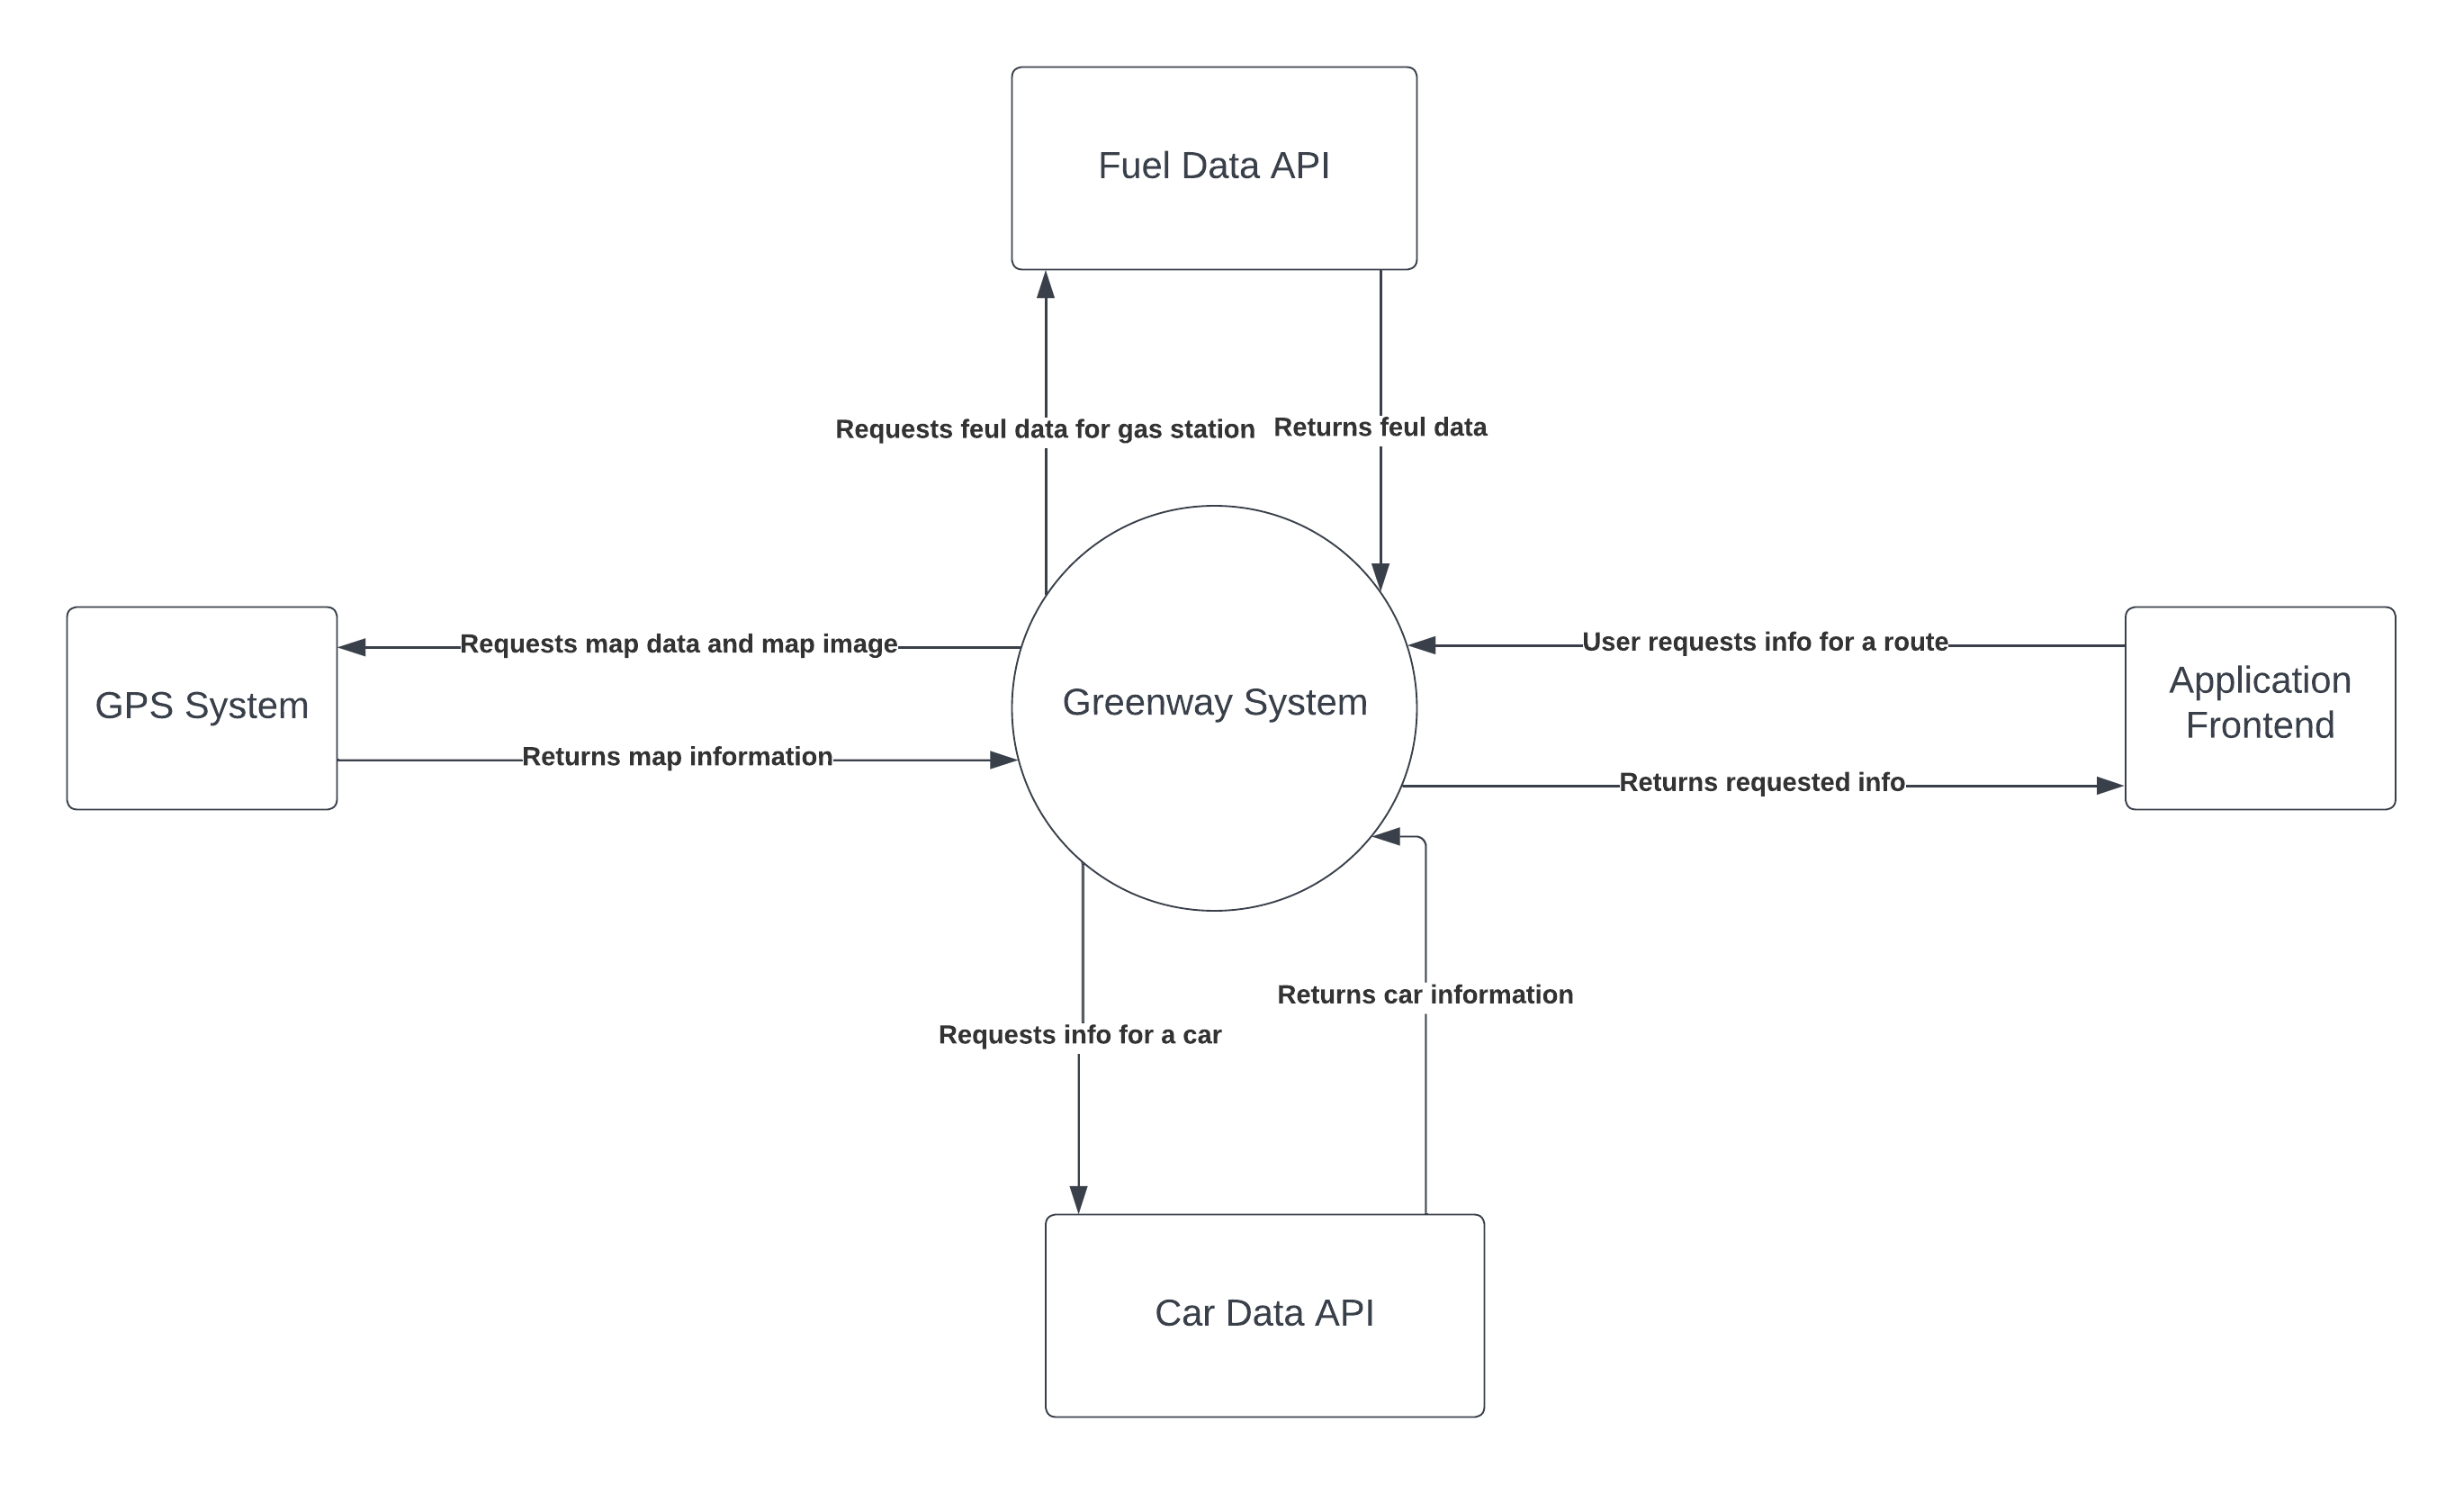
\includegraphics[width=0.8\textwidth]{ContextDiagram.png}
\caption{Context Diagram}
\label{Fig_SystemContext} 
\end{center}
\end{figure}


\begin{itemize}
\item User Responsibilities:
\begin{itemize}
\item Responsible for interacting with Application Frontend and receiving its output. 
\end{itemize}
\item \progname{} System Responsibilities:
\begin{itemize}
\item Responsible for calculating the total fuel price for trip with data from 
Feul Data API.
\item Responsible for interacting with GPS API to get all neccessary GPS data 
to present to user.
\item Responsible for interacting with Car Data API to get car information 
and process it.
\item Responsible for interacting with Charging station API to get charging 
station data.
\end{itemize}
\item Application Frontend Responsibilities:
\begin{itemize}
\item Responsible for allowing user to interact with application and displaying application output.
\end{itemize}
\item Fuel Data API Responsibilities:
\begin{itemize}
\item Responsible for sending Feul Station Data to any service requesting it.
\end{itemize}
\item GPS System Responsibilities:
\begin{itemize}
\item Responsible for sending any GPS data required to a service needing it.
\end{itemize}
\item Car Data API Responsibilities:
\begin{itemize}
\item Responsible for sending any Car data required to a service needing it.
\end{itemize}
\item Charging API Responsibilities:
\begin{itemize}
\item Responsible for sending any Charging Station data required to a service needing it.
\end{itemize}
\end{itemize}

\subsection{User Characteristics} \label{SecUserCharacteristics}

The users for this application will be individuals that are looking to drive electric 
cars, or already have them. As such this application serves individuals considering to 
transition to electric vehicles from gas vehicles, and will assume all users have basic 
familiarity with cars. This app will also support individuals in assessing the infrastructure 
surrounding electric cars to ease in the transition previously mentioned. Lastly, this app 
can also assist individuals that already own electric cars to find economic routes to reach 
their destination.

\section{Behavior}

\begin{figure}[h!]
  \begin{center}
   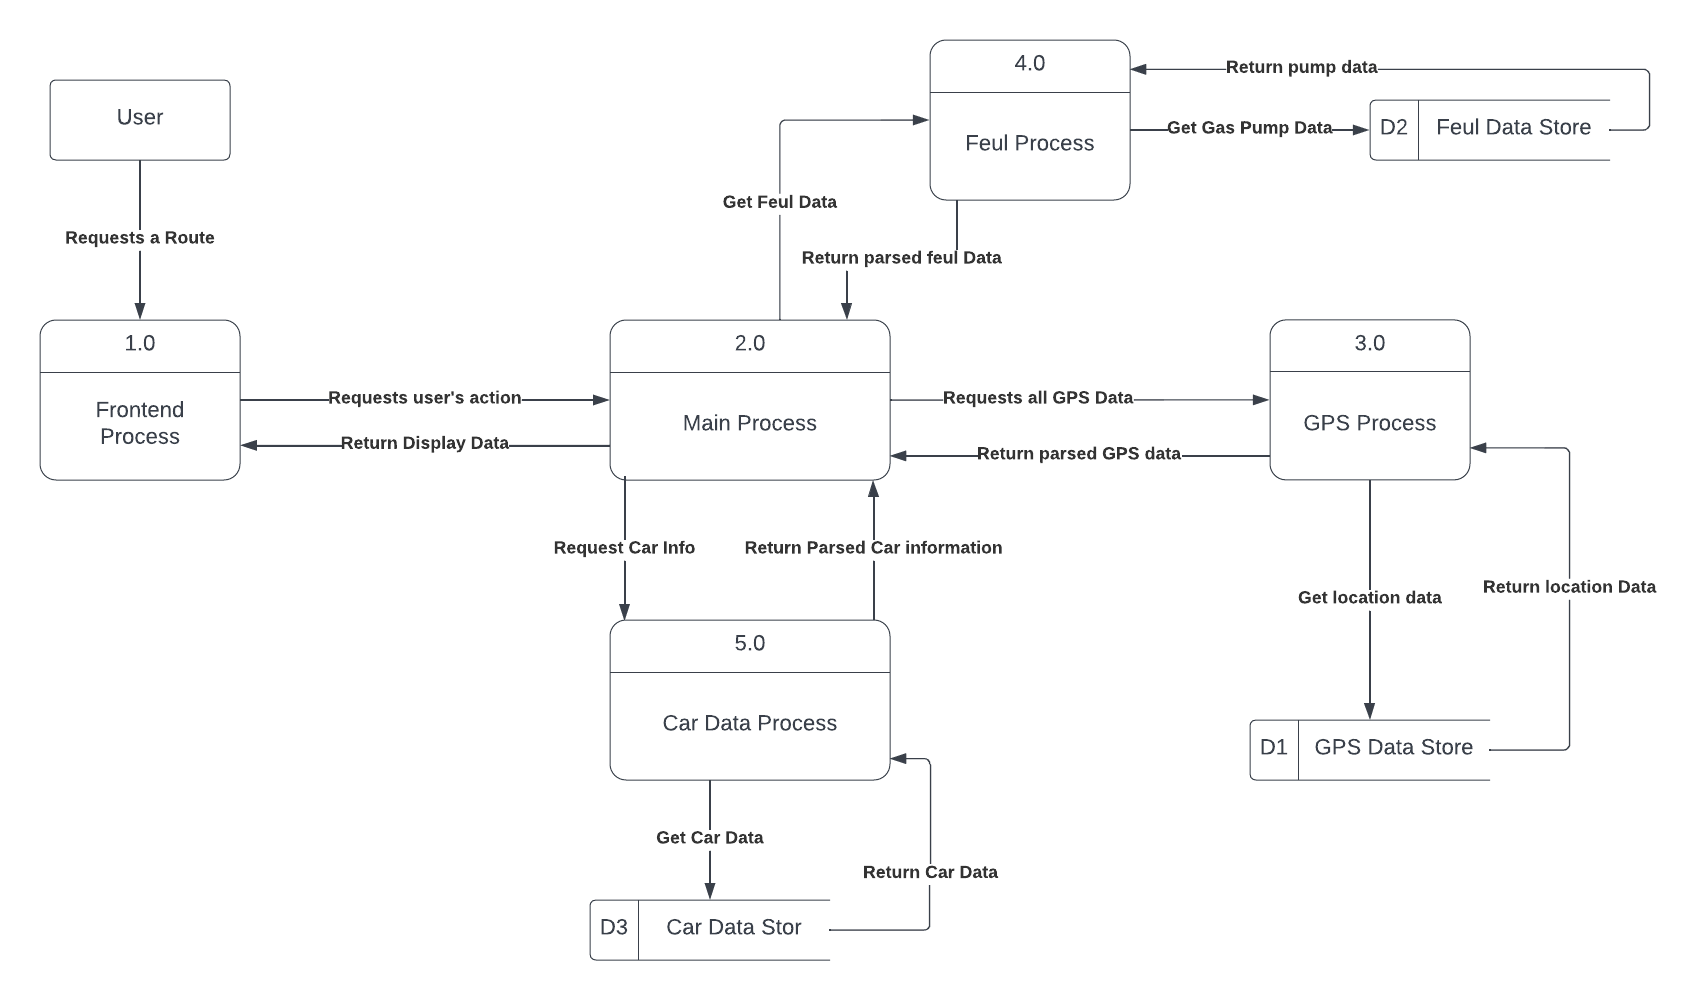
\includegraphics[width=0.8\textwidth]{DataFlowDiagram.png}
  \caption{Application Behavior from a Data Flow Diagram}
  \label{Fig_DataFlow} 
  \end{center}
\end{figure}

\section{Requirements}

\plt{The requirements refine the goal statement.  They will make heavy use of
  references to the instance models.}

This section provides the functional requirements, the business tasks that the
software is expected to complete, and the nonfunctional requirements, the
qualities that the software is expected to exhibit.

\subsection{Functional Requirements}

\noindent \begin{itemize}

\item[R\refstepcounter{reqnum}\thereqnum ] The system shall allow the user a way to input start location.

\item[R\refstepcounter{reqnum}\thereqnum ] The system shall allow the user a way to input final destination.

\item[R\refstepcounter{reqnum}\thereqnum ] The system shall allow the user a way to select car models.

\item[R\refstepcounter{reqnum}\thereqnum ] The system shall allow the user a way to input the custom details of their car.

\item[R\refstepcounter{reqnum}\thereqnum ] The system shall have a way to update available car models from either user input or external sources.

\item[R\refstepcounter{reqnum}\thereqnum ] The system shall have a map to show journey from start to final destination.

\item[R\refstepcounter{reqnum}\thereqnum ] The system shall display the gas stations along the route.

\item[R\refstepcounter{reqnum}\thereqnum ] The system shall display charging stations along the route for electric vehicles.

\item[R\refstepcounter{reqnum}\thereqnum ] The system shall have a way to collect gas prices on route to destination.

\item[R\refstepcounter{reqnum}\thereqnum ] The system shall have a way to calculate the most fuel efficient route.

\item[R\refstepcounter{reqnum}\thereqnum ] The system shall have a way to collect elevation data along the suggested route.

\item[R\refstepcounter{reqnum}\thereqnum ] The system shall have a way to calculate fuel consumption on different terrain elevations.

\item[R\refstepcounter{reqnum}\thereqnum ] The system shall have a way to calculate the total cost of the journey.

\end{itemize}

\subsection{Non-functional Requirements}

\noindent \begin{itemize}

\item[NFR\refstepcounter{nfrnum}\thenfrnum \label{NFR_1}:] 
\begin{itemize}
  \item \textit{Description}: The system shall have a modern minimalist user interface.
  \item \textit{Rationale}: Using popular modern design principles to create an appealing visual style for the system will make the system easy to use and attractive to users.
  \item \textit{Fit Criterion}: The system’s UI must follow modern minimalist design principles as defined in popular style guides. Users feedback will be used to assess the overall design of the interface. 
  \item \textit{Undesired Event Handling}: Given poor user feedback on interface design, user suggestions will be considered and overall interface design will be reevaluated. 
  \item \textit{Priority}: Medium
\end{itemize}


\item[NFR\refstepcounter{nfrnum}\thenfrnum \label{NFR_2}:] 
\begin{itemize}
  \item \textit{Description}: The system shall have a consistent style across the different pages (or interfaces) of the platform. 
  \item \textit{Rationale}: System will appear more professional. User experience will be more streamlined and less confusing if the system maintains a cohesive style. 
  \item \textit{Fit Criterion}: Each page/interface shall be checked against a list of common style/design elements that should remain consistent within the project. User feedback will be used to assess style consistency between interfaces. 
  \item \textit{Undesired Event Handling}: Given feedback on inconsistent style, alterations will be made to the interface to address specific feedback. 
  \item \textit{Priority}: Medium
\end{itemize}

\item[NFR\refstepcounter{nfrnum}\thenfrnum \label{NFR_3}:] 
\begin{itemize}
  \item \textit{Description}: The system shall have a user interface which is intuitive and easy to navigate. 
  \item \textit{Rationale}: Ease of use improves learnability and memorability of the system.
  \item \textit{Fit Criterion}: User feedback will be used to assess ease of use. Metrics such as time taken for new user to complete sample task will be measured.
  \item \textit{Undesired Event Handling}: Given poor ease of use metrics, the layout, simplicity, and flow of system will be reevaluated and alterations made. 
  \item \textit{Priority}: High
\end{itemize}

\item[NFR\refstepcounter{nfrnum}\thenfrnum \label{NFR_4}:] 
\begin{itemize}
  \item \textit{Description}: The system shall retain the user’s previous destinations. 
  \item \textit{Rationale}: Reduces time taken to select destination if user has frequently used destinations. Improves ease of use (NFR 3) by reducing time needed to complete task. 
  \item \textit{Fit Criterion}: Are the user’s previous destinations available to the user? Yes/No.  
  \item \textit{Undesired Event Handling}: If no, functionality should be implemented.
  \item \textit{Priority}: Medium
\end{itemize}

\item[NFR\refstepcounter{nfrnum}\thenfrnum \label{NFR_5}:] 
\begin{itemize}
  \item \textit{Description}: The system shall have a guide (or short tutorial) for those who are using the application for the first time. 
  \item \textit{Rationale}: The guide/tutorial will introduce how to use all the features offered by the system.
  \item \textit{Fit Criterion}: Several metrics measuring task completion will be compared: first time user without tutorial, first time user with tutorial, repeat user without tutorial. User feedback will also be obtained. Majority of users \(\>80\%\) should feel comfortable with system functionality after viewing the tutorial.  
  \item \textit{Undesired Event Handling}: Given poor learnability, tutorial/guide and overall layout and ease of use (NFR 3) shall be reevaluated and alterations made.
  \item \textit{Priority}: High
\end{itemize}

\item[NFR\refstepcounter{nfrnum}\thenfrnum \label{NFR_6}:] 
\begin{itemize}
  \item \textit{Description}: The system shall hide the details of its implementation from the user.
  \item \textit{Rationale}: The implementation (e.g. code, algorithms, etc.), is only relevant to the developers. Users are only concerned about the application functionality and outputs.
  \item \textit{Fit Criterion}: During software testing, developers can test to see if abstraction was properly used to hide the details of the implementation of the system from the user.  
  \item \textit{Undesired Event Handling}: Given poor abstraction, details will be hidden or omitted from the user interface. 
  \item \textit{Priority}: High
\end{itemize}

\item[NFR\refstepcounter{nfrnum}\thenfrnum \label{NFR_7}:] 
\begin{itemize}
  \item \textit{Description}: The system shall be accessible to users with visual impairments. 
  \item \textit{Rationale}: The system shall be accessible to users with visual impairments. 
  \item \textit{Fit Criterion}: The system will be tested in conditions where the user is partially or completely visually impaired. 
  \item \textit{Undesired Event Handling}: Given poor accessibility, modifications to the system will be made to improve the usability of the system under these conditions.
  \item \textit{Priority}: Medium
\end{itemize}

\item[NFR\refstepcounter{nfrnum}\thenfrnum \label{NFR_8}:] 
\begin{itemize}
  \item \textit{Description}: The system shall complete the route and fuel consumption calculation in a reasonable amount of time (<5 seconds). 
  \item \textit{Rationale}: The user should not have to wait a very long time after they input their destination into the application.
  \item \textit{Fit Criterion}: The time between the user input and the route calculation shall not exceed 5 seconds. The system calculation time should be comparable to the default google maps route calculation time.  
  \item \textit{Undesired Event Handling}: Given poor calculation time, algorithm time efficiency and other sources of lag should be considered and fixed (if possible). 
  \item \textit{Priority}: Low
\end{itemize}

\item[NFR\refstepcounter{nfrnum}\thenfrnum \label{NFR_9}:] 
\begin{itemize}
  \item \textit{Description}: The system shall calculate fuel consumption as accurately as possible.
  \item \textit{Rationale}: We want our customers to know exactly how much fuel will be consumed during the trip. It is vital that the value be accurate so that they can plan their trip accordingly.
  \item \textit{Fit Criterion}: In a panel of 50 users using the application, 80\% of the users are satisfied with the calculation.
  \item \textit{Undesired Event Handling}: N/A.
  \item \textit{Priority}: Medium
\end{itemize}

\item[NFR\refstepcounter{nfrnum}\thenfrnum \label{NFR_10}:] 
\begin{itemize}
  \item \textit{Description}: The system shall be available for use 24 hours per day, 365 days per year.
  \item \textit{Rationale}: Since this is a web app, it will be available for use at any time. Users will be able to use the application at any time of the day without any restriction.
  \item \textit{Fit Criterion}: 90\% of a panel of 10 users shall be able to use the application without it going offline.
  \item \textit{Undesired Event Handling}: N/A.
  \item \textit{Priority}: Low
\end{itemize}

\item[NFR\refstepcounter{nfrnum}\thenfrnum \label{NFR_11}:] 
\begin{itemize}
  \item \textit{Description}: The system shall be able to respond to invalid or unconventional inputs.  
  \item \textit{Rationale}: Ensures user error will not cause bugs or impede system functionality. 
  \item \textit{Fit Criterion}: Test cases with invalid inputs and outliers will be created to test this non-functional requirement.  
  \item \textit{Undesired Event Handling}: N/A. 
  \item \textit{Priority}: High
\end{itemize}

\end{itemize}

\section{Likely Changes}    

\noindent \begin{itemize}

\item[LC\refstepcounter{lcnum}\thelcnum\label{Long Journey}:] The addition of the application being able to use mileage data as well as gas tank size to calculate the most efficient route on a long journey, allowing for the least amount of stops to fill up gas.

\item[LC\refstepcounter{lcnum}\thelcnum\label{Electric Cars}:] The addition of the application taking data of electric cars to allow the use of not only gas station but charging stations for electric car users.

\item[LC\refstepcounter{lcnum}\thelcnum\label{Bigger Area}:] The application will be able to be used in all of Ontario with elevation and gas data for all areas.

\item[LC\refstepcounter{lcnum}\thelcnum\label{Application Integration}:] Future changes should allow the application to be used with other apps other than Google Maps, such as Wayz or Apple Maps.

\end{itemize}

\section{Unlikely Changes}    

\noindent \begin{itemize}

\item[ULC\refstepcounter{ulcnum}\theulcnum\label{Regional Support}:] The application will not support other provinces or countries.

\item[ULC\refstepcounter{ulcnum}\theulcnum\label{New Cars}:] The application will not be able to update car catalog information on its own and will require an update to the application when new cars are introduced.

\item[ULC\refstepcounter{ulcnum}\theulcnum\label{Hybrid Cars}:] The application will not support hybrid vehicles as they require complex calculations to determine when the electric component of the vehicle is used and when the gas component is.

\end{itemize}

\section{Traceability Matrices and Graphs}

The purpose of the traceability matrices is to provide easy references on what
has to be additionally modified if a certain component is changed.  Every time a
component is changed, the items in the column of that component that are marked
with an ``X'' may have to be modified as well.  Table~\ref{Table:trace} shows the
dependencies of theoretical models, general definitions, data definitions, and
instance models with each other. Table~\ref{Table:R_trace} shows the
dependencies of instance models, requirements, and data constraints on each
other. Table~\ref{Table:A_trace} shows the dependencies of theoretical models,
general definitions, data definitions, instance models, and likely changes on
the assumptions.

\plt{You will have to modify these tables for your problem.}

\plt{The traceability matrix is not generally symmetric.  If GD1 uses A1, that
  means that GD1's derivation or presentation requires invocation of A1.  A1
  does not use GD1.  A1 is ``used by'' GD1.}

\plt{The traceability matrix is challenging to maintain manually.  Please do
  your best.  In the future tools (like Drasil) will make this much easier.}

\afterpage{
\begin{landscape}
\begin{table}[h!]
\centering
\begin{tabular}{|c|c|c|c|c|c|c|c|c|c|c|c|c|c|c|c|c|c|c|c|}
\hline
	& \aref{A_OnlyThermalEnergy}& \aref{A_hcoeff}& \aref{A_mixed}& \aref{A_tpcm}& \aref{A_const_density}& \aref{A_const_C}& \aref{A_Newt_coil}& \aref{A_tcoil}& \aref{A_tlcoil}& \aref{A_Newt_pcm}& \aref{A_charge}& \aref{A_InitTemp}& \aref{A_OpRangePCM}& \aref{A_OpRange}& \aref{A_htank}& \aref{A_int_heat}& \aref{A_vpcm}& \aref{A_PCM_state}& \aref{A_Pressure} \\
\hline
\tref{T_COE}        & X& & & & & & & & & & & & & & & & & & \\ \hline
\tref{T_SHE}        & & & & & & & & & & & & & & & & & & & \\ \hline
\tref{T_LHE}        & & & & & & & & & & & & & & & & & & & \\ \hline
\dref{NL}           & & X& & & & & & & & & & & & & & & & & \\ \hline
\dref{ROCT}         & & & X& X& X& X& & & & & & & & & & & & & \\ \hline
\ddref{FluxCoil}    & & & & & & & X& X& X& & & & & & & & & & \\ \hline
\ddref{FluxPCM}     & & & X& X& & & & & & X& & & & & & & & & \\ \hline
\ddref{D_HOF}       & & & & & & & & & & & & & & & & & & & \\ \hline
\ddref{D_MF}        & & & & & & & & & & & & & & & & & & & \\ \hline
\iref{ewat}         & & & & & & & & & & & X& X& & X& X& X& & & X \\ \hline
\iref{epcm}         & & & & & & & & & & & & X& X& & & X& X& X& \\ \hline
\iref{I_HWAT}       & & & & & & & & & & & & & & X& & & & & X \\ \hline
\iref{I_HPCM}       & & & & & & & & & & & & & X& & & & & X & \\ \hline
\lcref{LC_tpcm}     & & & & X& & & & & & & & & & & & & & & \\ \hline
\lcref{LC_tcoil}    & & & & & & & & X& & & & & & & & & & & \\ \hline
\lcref{LC_tlcoil}   & & & & & & & & & X& & & & & & & & & & \\ \hline
\lcref{LC_charge}   & & & & & & & & & & & X& & & & & & & & \\ \hline
\lcref{LC_InitTemp} & & & & & & & & & & & & X& & & & & & & \\ \hline
\lcref{LC_htank}    & & & & & & & & & & & & & & & X& & & & \\
\hline
\end{tabular}
\caption{Traceability Matrix Showing the Connections Between Assumptions and Other Items}
\label{Table:A_trace}
\end{table}
\end{landscape}
}

\begin{table}[h!]
\centering
\begin{tabular}{|c|c|c|c|c|c|c|c|c|c|c|c|c|c|c|c|c|c|c|c|c|c|c|c|}
\hline        
	& \tref{T_COE}& \tref{T_SHE}& \tref{T_LHE}& \dref{NL}& \dref{ROCT} & \ddref{FluxCoil}& \ddref{FluxPCM} & \ddref{D_HOF}& \ddref{D_MF}& \iref{ewat}& \iref{epcm}& \iref{I_HWAT}& \iref{I_HPCM} \\
\hline
\tref{T_COE}     & & & & & & & & & & & & & \\ \hline
\tref{T_SHE}     & & & X& & & & & & & & & & \\ \hline
\tref{T_LHE}     & & & & & & & & & & & & & \\ \hline
\dref{NL}        & & & & & & & & & & & & & \\ \hline
\dref{ROCT}      & X& & & & & & & & & & & & \\ \hline
\ddref{FluxCoil} & & & & X& & & & & & & & & \\ \hline
\ddref{FluxPCM}  & & & & X& & & & & & & & & \\ \hline
\ddref{D_HOF}    & & & & & & & & & & & & & \\ \hline
\ddref{D_MF}     & & & & & & & & X& & & & & \\ \hline
\iref{ewat}      & & & & & X& X& X& & & & X& & \\ \hline
\iref{epcm}      & & & & & X& & X& & X& X& & & X \\ \hline
\iref{I_HWAT}    & & X& & & & & & & & & & & \\ \hline
\iref{I_HPCM}    & & X& X& & & & X& X& X& & X& & \\
\hline
\end{tabular}
\caption{Traceability Matrix Showing the Connections Between Items of Different Sections}
\label{Table:trace}
\end{table}

\begin{table}[h!]
\centering
\begin{tabular}{|c|c|c|c|c|c|c|c|}
\hline
	& \iref{ewat}& \iref{epcm}& \iref{I_HWAT}& \iref{I_HPCM}& \ref{sec_DataConstraints}& \rref{R_RawInputs}& \rref{R_MassInputs} \\
\hline
\iref{ewat}            & & X& & & & X& X \\ \hline
\iref{epcm}            & X& & & X& & X& X \\ \hline
\iref{I_HWAT}          & & & & & & X& X \\ \hline
\iref{I_HPCM}          & & X& & & & X& X \\ \hline
\rref{R_RawInputs}     & & & & & & & \\ \hline
\rref{R_MassInputs}    & & & & & & X& \\ \hline
\rref{R_CheckInputs}   & & & & & X& & \\ \hline
\rref{R_OutputInputs}  & X& X& & & & X& X \\ \hline
\rref{R_TempWater}     & X& & & & & & \\ \hline 
\rref{R_TempPCM}       & & X& & & & & \\ \hline
\rref{R_EnergyWater}   & & & X& & & & \\ \hline
\rref{R_EnergyPCM}     & & & & X& & & \\ \hline
\rref{R_VerifyOutput}  & & & X& X& & & \\ \hline
\rref{R_timeMeltBegin} & & X& & & & & \\ \hline
\rref{R_timeMeltEnd}   & & X& & & & & \\ 
\hline
\end{tabular}
\caption{Traceability Matrix Showing the Connections Between Requirements and Instance Models}
\label{Table:R_trace}
\end{table}

The purpose of the traceability graphs is also to provide easy references on
what has to be additionally modified if a certain component is changed.  The
arrows in the graphs represent dependencies. The component at the tail of an
arrow is depended on by the component at the head of that arrow. Therefore, if a
component is changed, the components that it points to should also be
changed. Figure~\ref{Fig_ATrace} shows the dependencies of theoretical models,
general definitions, data definitions, instance models, likely changes, and
assumptions on each other. Figure~\ref{Fig_RTrace} shows the dependencies of
instance models, requirements, and data constraints on each other.

% \begin{figure}[h!]
% 	\begin{center}
% 		%\rotatebox{-90}
% 		{
% 			\includegraphics[width=\textwidth]{ATrace.png}
% 		}
% 		\caption{\label{Fig_ATrace} Traceability Matrix Showing the Connections Between Items of Different Sections}
% 	\end{center}
% \end{figure}


% \begin{figure}[h!]
% 	\begin{center}
% 		%\rotatebox{-90}
% 		{
% 			\includegraphics[width=0.7\textwidth]{RTrace.png}
% 		}
% 		\caption{\label{Fig_RTrace} Traceability Matrix Showing the Connections Between Requirements, Instance Models, and Data Constraints}
% 	\end{center}
% \end{figure}

\section{Development Plan}

\plt{This section is optional.  It is used to explain the plan for developing
  the software.  In particular, this section gives a list of the order in which
  the requirements will be implemented.  In the context of a course  this is
  where you can indicate which requirements will be implemented as part of the
  course, and which will be ``faked'' as future work.  This section can be
  organized as a prioritized list of requirements, or it could should the
  requirements that will be implemented for ``phase 1'', ``phase 2'', etc.}

\section{Values of Auxiliary Constants}

\plt{Show the values of the symbolic parameters introduced in the report.}

\plt{The definition of the requirements will likely call for SYMBOLIC\_CONSTANTS.
Their values are defined in this section for easy maintenance.}

\plt{The value of FRACTION, for the Maintainability NFR would be given here.}

\newpage

\bibliographystyle {plainnat}
\bibliography {../../refs/References}

\newpage

\noindent \plt{The following is not part of the template, just some things to consider
  when filing in the template.}

\noindent \plt{Grammar, flow and \LaTeX advice:
\begin{itemize}
\item For Mac users \texttt{*.DS\_Store} should be in \texttt{.gitignore}
\item \LaTeX{} and formatting rules
\begin{itemize}
\item Variables are italic, everything else not, includes subscripts (link to
  document)
\begin{itemize}
\item \href{https://physics.nist.gov/cuu/pdf/typefaces.pdf}{Conventions}
\item Watch out for implied multiplication
\end{itemize}
\item Use BibTeX
\item Use cross-referencing
\end{itemize}
\item Grammar and writing rules
\begin{itemize}
\item Acronyms expanded on first usage (not just in table of acronyms)
\item ``In order to'' should be ``to''
\end{itemize}
\end{itemize}}

\noindent \plt{Advice on using the template:
\begin{itemize}
\item Difference between physical and software constraints
\item Properties of a correct solution means \emph{additional} properties, not
  a restating of the requirements (may be ``not applicable'' for your problem).
  If you have a table of output constraints, then these are properties of a
  correct solution.
\item Assumptions have to be invoked somewhere
\item ``Referenced by'' implies that there is an explicit reference
\item Think of traceability matrix, list of assumption invocations and list of
  reference by fields as automatically generatable
\item If you say the format of the output (plot, table etc), then your
  requirement could be more abstract
\end{itemize}
}

\newpage{}
\section*{Appendix --- Reflection}

There are many skills needed to accomplish the task, these skills however need to be distributed amongst the team as it makes it easier to complete the goals that have been set to acquire a finished product. The domain specific knowledge required ranges from understanding APIs to collecting, storing, and using data. The team requires the knowledge of how to collect the different types of data required, gas price data, elevation data of a specified area, car catalog data that contains information about gas mileage, and google maps data for fuel efficient route calculations. The intention is to use this data as a collective to perform calculations which would allow the user to find the cost of travel from one destination to another in the simplest manner; for this, an understanding of how the Google Maps API works, how the application will be developed, how the interface will be designed, and how everything will work simultaneously to provide the user with the best experience. These tasks are split amongst the team.

\bigskip

\noindent Jash --- Collection of gas price data and how it will be stored and how the fuel calculation will be performed.

\bigskip

\noindent Priyansh --- Collection of elevation specific data and how it will be stored and how the fuel calculation will be performed.

\bigskip

\noindent Utsharga --- Collection of car catalog data and how it will be stored and how the fuel calculation will be performed.

\bigskip

\noindent Sharjil --- Understanding of how the interface will be designed and how the fuel-efficient route will be calculated.

\bigskip

\noindent Bilal --- Understanding of how the Google Maps API works and how the fuel-efficient route will be calculated.

\bigskip

\noindent Pranay --- Understanding How the interface will be designed and how everything will work simultaneously.

\bigskip

There are many approaches to acquiring this knowledge; one approach is researching in the specific domain through forums and google searches. Another approach is getting hands on with the entity you would like to learn, this allows one to experience and interact with it, giving a greater understanding of how everything works.

\bigskip

\noindent Jash --- The approach for collecting gas price data will be through the research domain, this allows him to find information about the gas prices as well as learn how to collect and store them in a specific way. The same approach applies to the fuel calculations as understanding how its done and factoring in the elevation data is going to be used.

\bigskip

\noindent Priyansh --- The approach for collecting elevation data will be done through the research domain, this makes sure the data being collected is relevant to the information required to perform the fuel calculations. The same approach applies to the fuel calculations as understanding how its done and factoring in the elevation data is going to be used.

\bigskip

\noindent Utsharga --- The approach for collecting car catalog data will be done through the research domain, this allows him to collect all necessary data on all existing cars to be used in production. The same approach applies to the fuel calculations as understanding how its done and factoring in the elevation data is going to be used.

\bigskip

\noindent Sharjil --- The design of the user interface will be done through the hand-on domain, this allows him to interact with the product and test to see what works and what doesn’t. The calculations for the fuel-efficient route will be done through the research domain, this allows him to create and work on the algorithm required to perform the calculation.

\bigskip

\noindent Bilal --- The Google Maps API will require the hand-on domain to be used to explore how it works and how it will be used for the purposes of this application, this will allow him to learn what to do and how to use it for our needs. The calculations for the fuel-efficient route will be done through the research domain, this allows him to create and work on the algorithm required to perform the calculation.

\bigskip

\noindent Pranay --- The design of the user interface will be done through the hand-on domain, this allows him to interact with the product and test to see what works and what doesn’t. To get everything working together, he will have to look into the hand-on domain to be able to test and see how all the different parts will need to be integrated together to allow for the product to function as intended.


\end{document}